\section{Định nghĩa và tính chất của tích phân}

Các khái niệm quen thuộc như độ dài, diện tích, và thể tích đã xuất hiện từ rất sớm trong lịch sử loài người, gắn liền với nhu cầu thực tiễn về đo lường. Mặc dù chúng ta có thể hình dung một cách trực quan rằng đây là những ``số đo'' về kích thước hay ``độ lớn'' của một vật thể, việc đưa ra một định nghĩa toán học chặt chẽ cho chúng không hề đơn giản, đặc biệt là câu hỏi: ``Làm thế nào để định nghĩa diện tích một cách tổng quát?''

Đối với những hình học cơ bản, câu trả lời có vẻ dễ dàng. Diện tích của một hình chữ nhật được xác định bằng tích chiều dài và chiều rộng. Từ đó, ta có thể suy ra công thức cho diện tích tam giác, và xa hơn là bất kỳ đa giác nào bằng cách phân chia nó thành các tam giác nhỏ. Tuy nhiên, phương pháp này trở nên bất lực trước những hình có đường biên cong.

Về mặt lịch sử, việc sử dụng khái niệm diện tích trong thực tế thường dựa trên hai nguyên tắc cơ bản: 
\begin{enumerate}[label=(\arabic*)]
    \item Chọn một hình làm ``đơn vị'' đo.
    \item Diện tích có tính chất cộng tính, tức là diện tích của một hình ghép bằng tổng diện tích các hình thành phần.
\end{enumerate}
Cách tiếp cận này, tuy hữu ích, nhưng vẫn chưa đủ để giải quyết bài toán một cách tổng quát.

Phải đến thế kỷ 17, với sự phát triển của giải tích, nhu cầu về một phương pháp tổng quát và chính xác để định nghĩa và tính toán diện tích mới thực sự được giải quyết. Vấn đề này đã dẫn đến sự hình thành của một phép toán tổng quát hóa quá trình cộng, được gọi là \textbf{phép tính tích phân}. Dưới đây, chúng ta sẽ bắt đầu tìm hiểu một trong những cách tiếp cận nền tảng nhất để xây dựng khái niệm này, được biết đến với tên gọi \textbf{tích phân Riemann}.

\subsection{Định nghĩa tích phân}

Xét một hàm số $f$ không âm, $f: [a, b] \to \R$. Mục tiêu của chúng ta là xác định ``diện tích'' của miền phẳng giới hạn bởi đồ thị của hàm $f$, trục hoành, và hai đường thẳng đứng $x=a, x=b$. Ý tưởng cơ bản là xấp xỉ miền cong này bằng một tập hợp các hình chữ nhật đơn giản. Đáy của mỗi hình chữ nhật là một đoạn con của $[a,b]$ và chiều cao được xác định bởi một giá trị của hàm $f$ trên đoạn con đó. Ta kỳ vọng rằng, khi chúng ta sử dụng ngày càng nhiều hình chữ nhật (tức là làm cho các đáy ngày càng nhỏ), tổng diện tích của chúng sẽ tiến gần đến giá trị diện tích thực của miền đang xét (xem Hình \ref{fig:rectangle_approx}).

Ta có thể cụ thể hóa ý tưởng này như sau. Trước hết, ta thực hiện một phép phân hoạch đoạn $[a, b]$ bằng một dãy các điểm:
\[ a = x_0 < x_1 < x_2 < \dots < x_n = b. \]
Phép phân hoạch này chia đoạn $[a, b]$ thành $n$ đoạn con $[x_{i-1}, x_i]$, với $i = 1, 2, \dots, n$. Trên mỗi đoạn con $[x_{i-1}, x_i]$, ta chọn một điểm bất kỳ $x_i^*$ và gọi nó là \textit{điểm mẫu}. Giá trị $f(x_i^*)$ được xem là chiều cao đại diện cho đồ thị của hàm $f$ trên toàn bộ đoạn con đó. Khi đó, ta có thể xây dựng một hình chữ nhật với đáy là $[x_{i-1}, x_i]$ (có độ dài là $\Delta x_i = x_i - x_{i-1}$) và chiều cao là $f(x_i^*)$. Diện tích của hình chữ nhật này là $f(x_i^*) \Delta x_i$.

Tổng diện tích của tất cả các hình chữ nhật này, được gọi là \textbf{tổng Riemann}\footnote{khoảng năm 1854, Bernhard Riemann đã đưa ra một định nghĩa chính xác về khái niệm tích phân}, là một giá trị xấp xỉ cho diện tích của miền dưới đồ thị:
\[ \sum_{i=1}^{n} f(x_i^*) (x_i - x_{i-1}) \]
Quá trình này được minh họa trong Hình \ref{fig:riemann_sum}.

\begin{figure}[H]
    \centering
    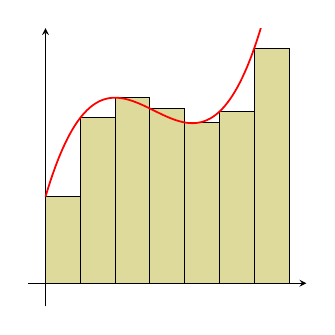
\begin{tikzpicture}[scale=0.8]
        \begin{axis}[
            axis lines=middle,
            xtick=\empty,
            ytick=\empty,
            xmin=-0.5, xmax=7.5,
            ymin=-0.5, ymax=5.5,
            width=6cm, height=6cm
        ]
        \addplot[ybar interval, fill=olive!30, domain=0:7, samples=8] {0.1 * (x-2)^3- 1/3 * (x-2)^2 + 4};
        \addplot[domain=0:7, samples=100, color=red, thick] {0.1 * (x-2)^3- 1/3 * (x-2)^2 + 4};
        \end{axis}
    \end{tikzpicture}
    \hspace{1cm}
    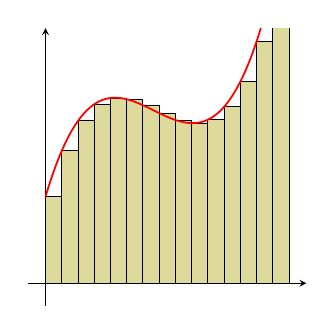
\begin{tikzpicture}[scale=0.8]
        \begin{axis}[
            axis lines=middle,
            xtick=\empty,
            ytick=\empty,
            xmin=-0.5, xmax=7.5,
            ymin=-0.5, ymax=5.5,
            width=6cm, height=6cm
        ]
        \addplot[ybar interval, fill=olive!30, domain=0:7, samples=16] {0.1 * (x-2)^3- 1/3 * (x-2)^2 + 4};
        \addplot[domain=0:7, samples=100, color=red, thick] {0.1 * (x-2)^3- 1/3 * (x-2)^2 + 4};
        \end{axis}
    \end{tikzpicture}
    \caption{Xấp xỉ diện tích bằng các hình chữ nhật.}
    \label{fig:rectangle_approx}
\end{figure}
\begin{figure}[H]
    \centering
    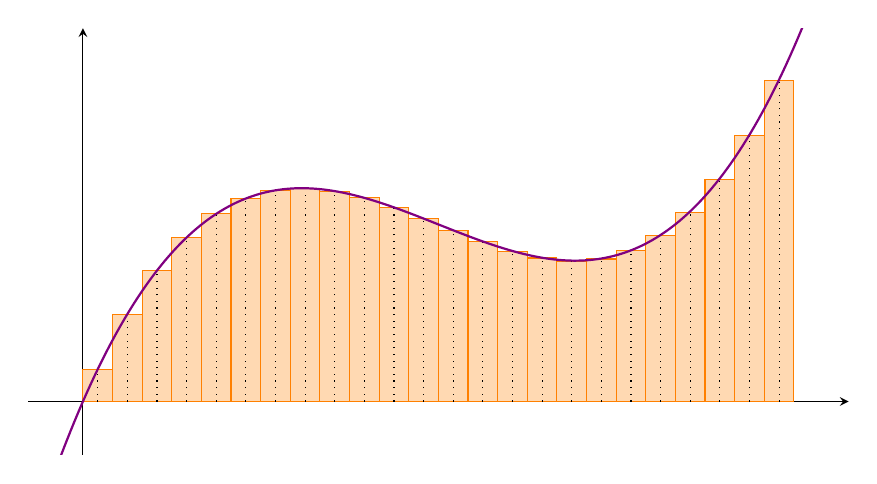
\begin{tikzpicture}[scale=1]
        \begin{axis}[
            axis lines=middle,
            xtick=\empty,
            ytick=\empty,
            xmin=-1, xmax=14,
            ymin=-1, ymax=7,
            width=12cm, height=7cm
        ]
        
        % Số cột
        \pgfmathsetmacro{\N}{24}
        % Bước chia
        \pgfmathsetmacro{\dx}{13/\N}
        
        % Vẽ các cột Riemann (lấy theo trung điểm)
        \foreach \i in {0,...,23} {
            \pgfmathsetmacro{\xmid}{(\i+0.5)*\dx} % trung điểm
            \pgfmathsetmacro{\y}{1/46*\xmid^3 - 39/92*\xmid^2 + 54/23*\xmid}
            % Hình chữ nhật (cột)
            \addplot[ybar, bar width=\dx, fill=orange!30, draw=orange] coordinates {(\xmid, \y)};
            % Đường chấm dọc
            \addplot[dotted, black] coordinates {(\xmid,0) (\xmid,\y)};
        }

        % Vẽ đường cong màu tím
        \addplot[domain=-0.8:13.5, samples=200, color=violet, thick] {1/46*x^3 - 39/92*x^2 + 54/23*x};
        
        \end{axis}
    \end{tikzpicture}
    \caption{Tổng Riemann (lấy theo trung điểm).}
    \label{fig:riemann_sum}
\end{figure}


\begin{example}
    Xét hàm số $f$ xác định bởi $f(x) = x^4 + 2$ trên đoạn $[1, 5]$. Ta sẽ tính xấp xỉ diện tích của miền dưới đồ thị hàm $f$.
    
    Ta xây dựng biểu thức tổng Riemann của $f$ trên $[1, 5]$ bằng cách chia đoạn này thành 8 đoạn con có độ dài bằng nhau, và chọn điểm mẫu là trung điểm của mỗi đoạn.
    
    Độ dài của mỗi đoạn con là $\Delta x = \dfrac{5-1}{8} = \dfrac{1}{2}$. Các điểm chia là $x_i = 1 + \dfrac{5-1}{8}i = 1 + \dfrac{i}{2}$ với $1 \le i \le 8$. Trung điểm của mỗi đoạn con $[x_{i-1}, x_i]$ là $x_i^* = 1 + \dfrac{5-1}{8}(i-1) + \dfrac{5-1}{16} = \dfrac{7}{8} + \dfrac{i}{2}$. Tổng Riemann tương ứng là:
    \[ \sum_{i=1}^{8} f(x_i^*) \Delta x = \sum_{i=1}^{8} \dfrac{1}{2} \left[ \left(\dfrac{7}{8} + \dfrac{i}{2}\right)^4 + 2 \right] \approx 645.34 \]
    Đây là một giá trị xấp xỉ cho diện tích của miền dưới đồ thị hàm $f(x) = x^4 + 2$ trên đoạn $[1, 5]$.
\end{example}

\begin{example}
    Một ô tô di chuyển trên một đường thẳng, với vận tốc tức thời tại thời điểm $t$ (đơn vị là km/h) là $v(t)$. Dữ liệu về vận tốc được ghi lại sau mỗi 15 phút như trong bảng sau:
    \begin{center}
    \begin{tabular}{|c|c|c|c|c|c|c|}
        \hline
        $t$ (giờ) & 0 & 0.25 & 0.5 & 0.75 & 1 & 1.25 \\
        \hline
        $v(t)$ (km/h) & 40 & 65 & 80 & 70 & 90 & 85 \\
        \hline
    \end{tabular}
    \end{center}
    Hãy ước lượng quãng đường mà ô tô đã đi được.

    Trên mỗi khoảng thời gian $[t_{i-1}, t_i]$, ta có thể xấp xỉ quãng đường đi được bằng cách lấy vận tốc ở đầu khoảng thời gian nhân với độ dài của khoảng thời gian đó: $v(t_{i-1})(t_i - t_{i-1})$. Tổng quãng đường đi được ước tính là:
    \[ 40 \cdot 0.25 + 65 \cdot 0.25 + 80 \cdot 0.25 + 70 \cdot 0.25 + 90 \cdot 0.25 = 86.25 \text{ km}. \]
    
    Tương tự, ta có thể xấp xỉ bằng cách sử dụng vận tốc ở cuối mỗi khoảng thời gian:
    \[ 65 \cdot 0.25 + 80 \cdot 0.25 + 70 \cdot 0.25 + 90 \cdot 0.25 + 85 \cdot 0.25 = 97.5 \text{ km}. \]
    Hai cách tính cho ra hai kết quả khác nhau. Ta hy vọng rằng có một giá trị chính xác cho quãng đường, và các giá trị trên chỉ là những xấp xỉ. Khi ta thu thập dữ liệu với các khoảng thời gian nhỏ hơn, các giá trị xấp xỉ sẽ tiến gần hơn đến giá trị thực.
\end{example}

\begin{example}
    Tốc độ quang hợp của một loài thực vật, ký hiệu là $P$, được đo bằng lượng $CO_2$ (tính bằng micromol trên mét vuông mỗi giây) mà lá cây hấp thụ. Dữ liệu thu thập được tại các thời điểm $t$ (tính bằng giây) như sau:
    \begin{center}
    \begin{tabular}{|c|c|c|c|c|c|c|}
        \hline
        $t$ & 0 & 15 & 30 & 45 & 60 & 75 \\
        \hline
        $P(t)$ & 3.1 & 4.5 & 5.2 & 6.1 & 5.8 & 5.3 \\
        \hline
    \end{tabular}
    \end{center}
    Ta muốn tính tổng lượng $CO_2$ mà một mét vuông lá cây hấp thụ được trong 75 giây đầu tiên.
    
    Nếu ta sử dụng giá trị đo ở đầu mỗi khoảng thời gian làm đại diện, ta có ước lượng:
    \[ 3.1 \cdot 15 + 4.5 \cdot 15 + 5.2 \cdot 15 + 6.1 \cdot 15 + 5.8 \cdot 15 = 370.5 \text{ micromol/m}^2. \]
    
    Nếu ta sử dụng giá trị đo ở cuối mỗi khoảng, ta có:
    \[ 4.5 \cdot 15 + 5.2 \cdot 15 + 6.1 \cdot 15 + 5.8 \cdot 15 + 5.3 \cdot 15 = 396 \text{ micromol/m}^2. \]
    Các ví dụ trên minh họa cho một ý tưởng chung: để tính một \textbf{tổng giá trị} của hàm $f$ trên một đoạn $I = [a, b]$, ta có thể chia nhỏ $I$ thành các đoạn con. Trên mỗi đoạn con, sự thay đổi của hàm $f$ sẽ ít hơn, do đó ta có thể xấp xỉ $f$ bằng một hằng số, chẳng hạn giá trị $f(x_i^*)$ tại một điểm mẫu. Tổng giá trị của $f$ trên đoạn $[x_{i-1}, x_i]$ được xấp xỉ bởi $f(x_i^*)(x_i - x_{i-1})$, và do đó, tổng giá trị trên toàn bộ đoạn $I$ được xấp xỉ bởi tổng Riemann:
    \[ \sum_{i=1}^{n} f(x_i^*) (x_i - x_{i-1}). \]
    Ta kỳ vọng rằng khi phép chia đoạn càng mịn (các đoạn con càng nhỏ), giá trị xấp xỉ sẽ càng tốt hơn, và giới hạn của quá trình này sẽ cho ta giá trị chính xác.
\end{example}

Để hiểu ``giới hạn'' của tổng Riemann một cách chính xác, ta nói rằng giới hạn đó là một số thực $L$ mà mọi tổng Riemann đều có thể tiến gần đến $L$ một cách tùy ý, miễn là phép chia đủ mịn.

\begin{definition}
    Giả sử tồn tại một số thực $L$ sao cho với mọi số thực $\epsilon > 0$, có một số thực $\delta > 0$ để với mọi phép chia
    \[ a = x_0 < x_1 < x_2 < \dots < x_n = b \]
    mà độ dài của mỗi đoạn $[x_{i-1}, x_i]$ đều nhỏ hơn $\delta$, và với mọi cách chọn điểm mẫu $x_i^* \in [x_{i-1}, x_i]$, ta luôn có:
    \[ \left| \sum_{i=1}^{n} f(x_i^*) (x_i - x_{i-1}) - L \right| < \epsilon. \]
    Số thực $L$ (nếu tồn tại) là duy nhất và được gọi là \textbf{tích phân} của $f$ trên $[a, b]$, ký hiệu là
    \[ \int_{a}^{b} f \quad \text{hoặc} \quad \int_{a}^{b} f(x) \dd x. \]
\end{definition}

Ký hiệu $\dd x$ trong tích phân chủ yếu để chỉ rõ biến số lấy tích phân và thường không có ý nghĩa độc lập. Nếu tích phân của $f$ tồn tại, ta nói hàm $f$ \textbf{có tích phân} hoặc \textbf{khả tích}. Khi $f$ khả tích, ta có thể tính xấp xỉ tích phân của nó với độ chính xác mong muốn bằng cách tính tổng Riemann.

\begin{definition}
    Nếu hàm $f$ không âm và khả tích trên đoạn $[a, b]$, ta định nghĩa \textbf{diện tích} của miền phẳng nằm dưới đồ thị của $f$ và trên trục $x$ là:
    \[ \int_{a}^{b} f(x) \dd x. \]
\end{definition}

% TODO: Sửa lại tham chiếu
Chúng ta sẽ quay lại vấn đề diện tích một cách chi tiết hơn trong Mục  \ref{sec:integral_applications}. Ta mở rộng định nghĩa của ký hiệu tích phân như sau. Với $a < b$, ta định nghĩa:
\[ \int_{b}^{a} f(x) \dd x = - \int_{a}^{b} f(x) \dd x. \]
Và ta cũng quy ước:
\[ \int_{a}^{a} f(x) \dd x = 0. \]

\subsection{Tính chất của tích phân}

Các tính chất sau đây được suy ra trực tiếp từ định nghĩa của tích phân thông qua tổng Riemann.

\begin{proposition} (Các tính chất cơ bản của tích phân)
    \begin{enumerate}[label=(\alph*)]
        \item Tích phân nếu tồn tại thì là duy nhất.
        
        \item Nếu $k$ là một hằng số thực và hàm $f$ có tích phân thì hàm $kf$ cũng có tích phân và
        \[ \int_{a}^{b} [k f(x)] \dd x = k \int_{a}^{b} f(x) \dd x. \]
        
        \item Nếu các hàm $f$ và $g$ đều có tích phân thì tổng $f+g$ cũng có tích phân và
        \[ \int_{a}^{b} [f(x) + g(x)] \dd x = \int_{a}^{b} f(x) \dd x + \int_{a}^{b} g(x) \dd x. \]
        
        \item Nếu hàm $f$ có tích phân trên các đoạn $[a, c]$ và $[c, b]$ thì $f$ cũng có tích phân trên $[a, b]$ và
        \[ \int_{a}^{c} f(x) \dd x + \int_{c}^{b} f(x) \dd x = \int_{a}^{b} f(x) \dd x. \]
        
        \item Nếu $f(x) \ge g(x)$ với mọi $x \in [a, b]$ thì
        \[ \int_{a}^{b} f(x) \dd x \ge \int_{a}^{b} g(x) \dd x. \]
    \end{enumerate}
\end{proposition}

Một số tính chất này có thể được giải thích và minh họa một cách trực quan thông qua ý nghĩa hình học. Chẳng hạn, tính chất (d) có thể hiểu là diện tích miền dưới đồ thị của $f$ trên đoạn $[a, b]$ bằng tổng diện tích trên các đoạn $[a, c]$ và $[c, b]$. Tương tự, tính chất (e) cho thấy nếu đồ thị của $f$ cao hơn đồ thị của $g$, thì diện tích tương ứng cũng lớn hơn.

\begin{proof}
    (a) Các tổng Riemann không thể cùng lúc tiến gần đến hai số thực khác nhau.
    
    (b) Đặt $\int_a^b f(x) \dd x = M$. Khi tổng Riemann của $f$ tiến gần đến $M$ một cách tùy ý, thì tổng Riemann của $kf$ cũng sẽ tiến gần đến $kM$ một cách tùy ý.
    
    (c) Đặt $\int_a^b g(x) \dd x = N$. Ta xét tổng Riemann của $f+g$ như sau, với $\Delta x_i = x_i - x_{i-1}$:
    \begin{align*}
        \left| \sum_{i} (f(x_i^*) + g(x_i^*))\Delta x_i - (M+N) \right| &= \left| \left(\sum_i f(x_i^*)\Delta x_i - M\right) + \left(\sum_i g(x_i^*)\Delta x_i - N\right) \right| \\
        &\le \left| \sum_i f(x_i^*)\Delta x_i - M \right| + \left| \sum_i g(x_i^*)\Delta x_i - N \right|.
    \end{align*}
    Điều này cho thấy nếu tổng Riemann của $f$ gần $M$ và tổng Riemann của $g$ gần $N$ thì tổng Riemann của $f+g$ sẽ gần $M+N$.
    
    (e) Nếu $f \ge g$ thì mọi tổng Riemann của $f$ sẽ lớn hơn hoặc bằng tổng Riemann tương ứng của $g$, tức là $\sum_i f(x_i^*)\Delta x_i \ge \sum_i g(x_i^*)\Delta x_i$.
\end{proof}

Từ cách xây dựng tích phân, có thể thấy rằng tính liên tục của hàm là một điều kiện rất quan trọng để đảm bảo phép xấp xỉ có hiệu quả. Nói một cách đơn giản, tính liên tục đảm bảo rằng khi biến số thay đổi nhỏ thì giá trị của hàm cũng thay đổi nhỏ, nhờ đó việc xấp xỉ giá trị hàm bằng cách lấy một giá trị đại diện trở nên chính xác hơn. Kết quả dưới đây khẳng định rằng tất cả các hàm liên tục đều khả tích.

\begin{theorem}[Hàm liên tục thì có tích phân]
    Nếu hàm $f$ liên tục trên đoạn $[a, b]$ thì tích phân $\int_a^b f$ tồn tại.
\end{theorem}

Có thể tìm thấy chứng minh chi tiết mệnh đề trên trong các tài liệu như
[TPTT02], [Spi94].

\subsection{Bài tập}

\begin{exercise}
    Một người đi xe đạp ghi lại vận tốc của mình (mét/giây) tại các thời điểm khác nhau (giây) trong 10 giây đầu tiên như sau:
    \begin{center}
    \begin{tabular}{|c|c|c|c|c|c|c|}
        \hline
        $t$ (giây) & 0 & 2 & 4 & 6 & 8 & 10 \\
        \hline
        $v(t)$ (m/s) & 0 & 1.5 & 2.5 & 3.0 & 2.5 & 2.0 \\
        \hline
    \end{tabular}
    \end{center}
    Hãy ước tính tổng quãng đường người đó đi được bằng hai cách:
    \begin{enumerate}[label=(\alph*)]
        \item Sử dụng vận tốc ở đầu mỗi khoảng thời gian (tổng Riemann trái).
        \item Sử dụng vận tốc ở cuối mỗi khoảng thời gian (tổng Riemann phải).
    \end{enumerate}
\end{exercise}

\begin{exercise}
    Cho hàm số $f$ liên tục trên đoạn $[0, 8]$. Bảng dưới đây cung cấp một số giá trị của hàm $f$:
    \begin{center}
    \begin{tabular}{|c|c|c|c|c|c|}
        \hline
        $x$ & 0 & 2 & 4 & 6 & 8 \\
        \hline
        $f(x)$ & 1.2 & 2.8 & 4.0 & 3.5 & 2.0 \\
        \hline
    \end{tabular}
    \end{center}
    Hãy tính xấp xỉ tích phân $\int_{0}^{8} f(x) \dd x$ bằng cách sử dụng tổng Riemann với 4 đoạn con có độ dài bằng nhau và lấy điểm mẫu là điểm cuối bên phải của mỗi đoạn.
\end{exercise}

\begin{exercise}
    Hãy tính tổng Riemann cho hàm số $f(x) = x^4$ trên đoạn $[0, 1]$ bằng cách chia đoạn này thành 5 đoạn con có độ dài bằng nhau và chọn điểm mẫu là trung điểm của mỗi đoạn.
\end{exercise}

\begin{exercise}
    Tính tổng Riemann cho hàm số $f(x) = \cos(\frac{\pi x}{8})$ trên đoạn $[0, 4]$, sử dụng 8 đoạn con có độ dài bằng nhau và lấy điểm mẫu là điểm đầu bên trái của mỗi đoạn.
\end{exercise}

\begin{exercise}
    Dựa vào đồ thị của hàm số $f$ trong hình dưới đây, hãy ước lượng diện tích của miền giới hạn bởi đồ thị và trục hoành trên đoạn $[0, 5]$.
    \begin{figure}[H]
        \centering
        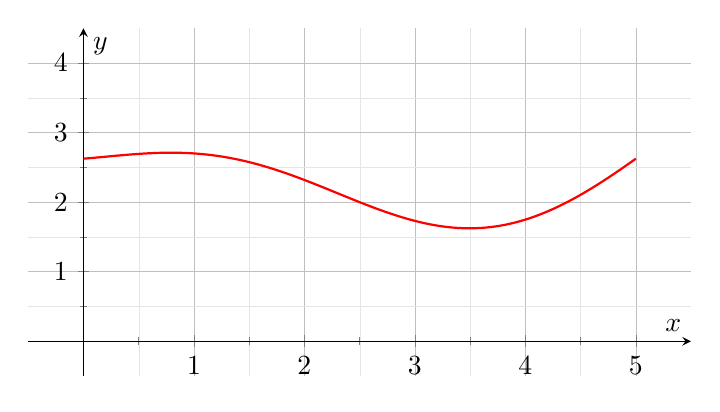
\begin{tikzpicture}[scale=1]
            \begin{axis}[
                axis lines=middle,
                grid=both,
                minor tick num=1,
                grid style={line width=.1pt, draw=gray!20},
                major grid style={line width=.2pt,draw=gray!50},
                xtick={0,1,2,3,4,5},
                ytick={0,1,2,3,4},
                xmin=-0.5, xmax=5.5,
                ymin=-0.5, ymax=4.5,
                width=10cm, height=6cm,
                xlabel=$x$,
                ylabel=$y$
            ]
            \addplot[domain=0:5, samples=100, color=red, thick, smooth] {2 + 0.5*sin(deg(x*pi/2.5)) + 0.1*(x-2.5)^2};
            \end{axis}
        \end{tikzpicture}
        \caption{Đồ thị của hàm số $f$ cho Bài tập 5.1.5.}
    \end{figure}
\end{exercise}

\begin{exercise}
    Sử dụng các tính chất của tích phân để chứng minh bất đẳng thức sau mà không cần tính giá trị của các tích phân:
    \[ \int_{0}^{1} \sqrt{1+x^2} \dd x \le \int_{0}^{1} \sqrt{1+x} \dd x. \]
    Gợi ý: So sánh hai hàm số $x^2$ và $x$ trên đoạn $[0, 1]$.
\end{exercise}

\begin{exercise}
    Sử dụng tính chất so sánh của tích phân để kiểm tra ước lượng sau:
    \[ 2 \le \int_{-1}^{1} \sqrt{1+x^4} \dd x \le 2\sqrt{2}. \]
\end{exercise}

\begin{exercise}
    Tìm một chặn trên và một chặn dưới cho tích phân sau:
    \[ \int_{0}^{2} \frac{1}{x^3+1} \dd x. \]
\end{exercise}

\begin{exercise}[*]
    Giả sử $f$ là một hàm liên tục trên đoạn $[a, b]$ và $f(x) \ge 0$ với mọi $x \in [a, b]$. Hãy giải thích tại sao nếu $\int_{a}^{b} f(x) \dd x = 0$ thì ta phải có $f(x) = 0$ với mọi $x \in [a, b]$.
\end{exercise}

\begin{exercise}
    Theo định luật Hooke, lực cần thiết để kéo dãn một lò xo thêm $x$ đơn vị so với chiều dài tự nhiên của nó là $F(x) = kx$, trong đó $k$ là hằng số lò xo. Giả sử một lò xo có chiều dài tự nhiên là 20 cm. Nếu cần một lực 50 N để giữ lò xo ở chiều dài 30 cm, hãy tính công thực hiện khi kéo lò xo từ chiều dài 30 cm đến 40 cm.
    
    (Gợi ý: Công được tính bằng tích phân của lực theo quãng đường dịch chuyển, $W = \int_a^b F(x) \dd x$).
\end{exercise}
